\section{迷宮入口 (entrance)}

\subsection{問題描述}

勇者林克要找尋傳說中的寶劍。
寶劍被封印在地下迷宮的深處,而要進入地下迷宮,必須在特定的地方詠唱咒文。
迷宮的入口附近有 \begin{math}n\end{math}
個圖騰,詠唱咒文產生的聲波必須恰好傳遞至「奇數」個圖騰,迷宮的入口才能開啟。
以二維座標平面來看,已知圖騰位置在格子點
\begin{math}P_1, P_2, \ldots, P_n\end{math}
上,且詠唱咒文能傳遞的範圍為一半徑為 \begin{math}r\end{math}
的圓(包含圓周),請計算座標平面上有幾個格子點在其上詠唱咒文能開啟迷宮入口。

以下圖為例,\begin{math}P_1, P_2, P_3\end{math}
為圖騰所在位置,每個小方格的邊長為
\begin{math}1\end{math}。若詠唱咒文的傳遞範圍為
\begin{math}2\end{math},則符合所求的格子點為圖上圓點所在的位置以及
\begin{math}P_1\end{math},共 \begin{math}17\end{math} 個點。

\begin{figure}[h]
\centering
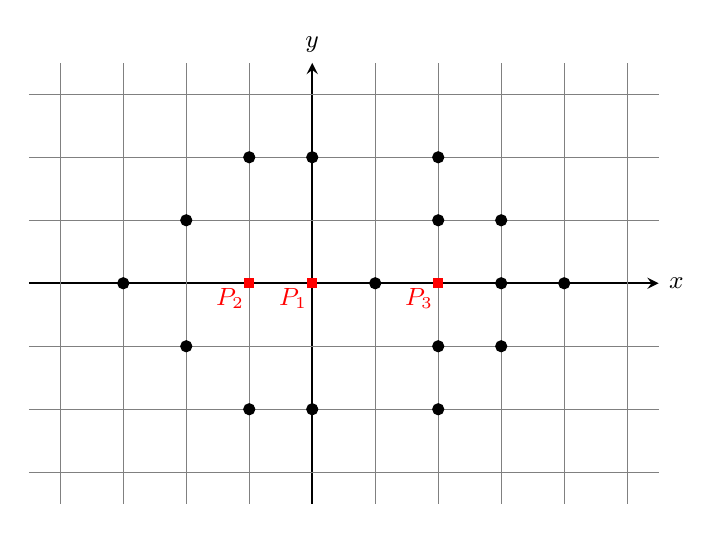
\begin{tikzpicture}[scale=0.8]
   \draw [-stealth,thick,black] (-4.5,0) -- (5.5,0) node[anchor=west]{\small$x$};
   \draw [-stealth,thick,black] (0,-3.5) -- (0,3.5) node[anchor=south]{\small$y$};
   \foreach \i in {-4,...,-1} {
      \draw [very thin,gray] (\i,-3.5) -- (\i,3.5);
   }
   \foreach \i in {1,...,5} {
      \draw [very thin,gray] (\i,-3.5) -- (\i,3.5);
   }
   \foreach \i in {-3,-2,-1} {
      \draw [very thin,gray] (-4.5,\i) -- (5.5,\i);
   }
   \foreach \i in {1,2,3} {
      \draw [very thin,gray] (-4.5,\i) -- (5.5,\i);
   }
   \filldraw[red] ([xshift=-2pt,yshift=-2pt]0, 0) rectangle ++(4pt,4pt) node[anchor=north east]{\small$P_1$};
   \filldraw[red] ([xshift=-2pt,yshift=-2pt]-1, 0) rectangle ++(4pt,4pt) node[anchor=north east]{\small$P_2$};
   \filldraw[red] ([xshift=-2pt,yshift=-2pt]2, 0) rectangle ++(4pt,4pt) node[anchor=north east]{\small$P_3$};
   \filldraw[black] (-3, 0) circle (2.5pt);
   \filldraw[black] (-2, -1) circle (2.5pt);
   \filldraw[black] (-2, 1) circle (2.5pt);
   \filldraw[black] (-1, -2) circle (2.5pt);
   \filldraw[black] (-1, 2) circle (2.5pt);
   \filldraw[black] (0, -2) circle (2.5pt);
   \filldraw[black] (0, 2) circle (2.5pt);
   \filldraw[black] (1, 0) circle (2.5pt);
   \filldraw[black] (2, -2) circle (2.5pt);
   \filldraw[black] (2, -1) circle (2.5pt);
   \filldraw[black] (2, 1) circle (2.5pt);
   \filldraw[black] (2, 2) circle (2.5pt);
   \filldraw[black] (3, -1) circle (2.5pt);
   \filldraw[black] (3, 0) circle (2.5pt);
   \filldraw[black] (3, 1) circle (2.5pt);
   \filldraw[black] (4, 0) circle (2.5pt);
\end{tikzpicture}
\end{figure}

\subsection{輸入格式}

\begin{format}
\f{
$n$ $r$
$x_1$ $y_1$
$x_2$ $y_2$
\vdots
$x_n$ $y_n$
}
\end{format}

\begin{itemize}
\tightlist
\item
  \begin{math}n\end{math} 為圖騰數量
\item
  \begin{math}r\end{math} 為咒文傳遞範圍的距離
\item
  \begin{math}(x_i, y_i)\end{math} 為第 \begin{math}i\end{math}
  個圖騰的位置 \begin{math}P_i\end{math}
\end{itemize}

\subsection{輸出格式}

\begin{format}
\f{
$\textrm{ans}$
}
\end{format}

\begin{itemize}
\tightlist
\item
  \begin{math}\textrm{ans}\end{math} 為一整數,代表滿足條件的格子點數量
\end{itemize}

\subsection{測資限制}

\begin{itemize}
\tightlist
\item
  \begin{math}1 \le n \le 2500\end{math}
\item
  \begin{math}1 \le r \le 10\end{math}
\item
  \begin{math}-10^6 \le x_i \le 10^6\end{math}
\item
  \begin{math}-10^6 \le y_i \le 10^6\end{math}
\item
  對於所有的 \begin{math}i\ne j\end{math},皆有
  \begin{math}P_i\ne P_j\end{math},亦即圖騰位置兩兩相異
\item
  輸入的數皆為整數
\end{itemize}

\subsection{範例測試}

\begin{example}
\exmp{
3 2
0 0
-1 0
2 0
}{%
17
}%
\end{example}

\subsection{評分說明}

本題共有三組子任務,條件限制如下所示。
每一組可有一或多筆測試資料,該組所有測試資料皆需答對才會獲得該組分數。

\begin{longtable}[]{@{}ccl@{}}
\toprule
子任務 & 分數 & 額外輸入限制 \\
\midrule
\endhead
1 & \(26\) & \begin{math}n = 1\end{math} \\
2 & \(36\) & \begin{math}|x_i|\le100\end{math} 且
\begin{math}|y_i|\le100\end{math} \\
3 & \(38\) & 無額外限制 \\
\bottomrule
\end{longtable}

\section{打鍵盤 (keyboard)}

\subsection{問題描述}

W
教授打字時只會使用左手與右手的食指,今天他打算打一篇僅由英文大寫字母構成的文章。
初始左手食指放在 F 上,右手食指放在 J 上。
每次要打一個字母時,可選擇用左手的食指或右手的食指輸入;輸入完該字母後,選用的食指就會停留在該按鍵的上方,另一根食指則停留在原按鍵的上方。

鍵盤如下圖,每個按鍵至多有 \begin{math}6\end{math} 個相鄰按鍵,
分別位於該按鍵的「左」、「右」、「左上」、「右上」、「左下」、「右下」六個方向。
食指在移動時,僅能依上述六個方向逐步移動,直到達到目標的字母為止。

\begin{figure}[h]
\centering
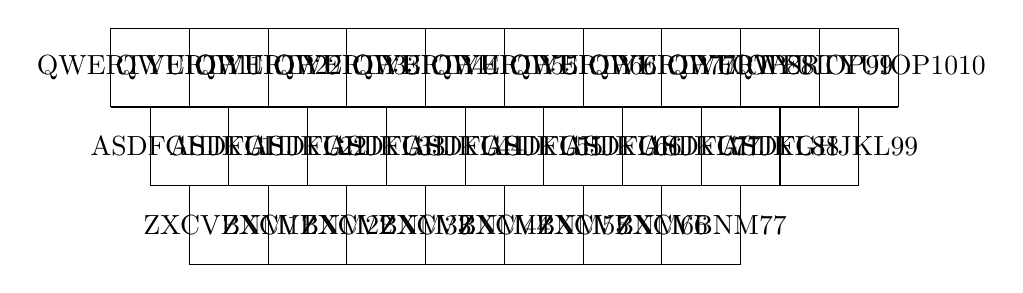
\begin{tikzpicture}[scale=0.5]
  \draw[step=2.0,black] (0,4) grid (20,6);
  \draw[step=2.0,black,xshift=-1cm] (2,2) grid (20,4);
  \draw[step=2.0,black] (2,0) grid (16,2);

  \def \s {QWERTYUIOP}
  \foreach \i in {1,...,10} {
    \node at (\i*2-1, 5) {\pdfsubstr{\s}{\i}{\i}};
  }

  \def \s {ASDFGHJKL}
  \foreach \i in {1,...,9} {
    \node at (\i*2, 3) {\pdfsubstr{\s}{\i}{\i}};
  }

  \def \s {ZXCVBNM}
  \foreach \i in {1,...,7} {
    \node at (\i*2+1, 1) {\pdfsubstr{\s}{\i}{\i}};
  }
\end{tikzpicture}
\end{figure}

已知 W 教授一次只會移動一根手指,手指移動到相鄰的按鍵需花
\begin{math}1\end{math}
單位時間,而其他動作的時間皆可忽略不計,請幫他計算打完這篇文章至少需要花多少單位時間。

舉例來說,若文章僅有 N 一個字母,使用左手食指從 F 移動至 N, 選擇
F→C→V→B→N 的移動路線所需的時間為 \begin{math}4\end{math} 單位,而選擇
F→G→H→N 所需的時間為 \begin{math}3\end{math} 單位。
耗時最短的移動路線為使用右手食指,直接由 J 移動至 N,所需的時間僅為
\begin{math}1\end{math} 單位,故答案為 \begin{math}1\end{math}。

\subsection{輸入格式}

\begin{format}
\f{
$n$
$S$
}
\end{format}

\begin{itemize}
\tightlist
\item
  \begin{math}n\end{math} 代表要輸入的文章長度
\item
  \begin{math}S\end{math} 為一字串,代表要輸入的文章
\end{itemize}

\subsection{輸出格式}

\begin{format}
\f{
$T$
}
\end{format}

\begin{itemize}
\tightlist
\item
  \begin{math}T\end{math} 為整數,代表 W 教授打完文章的最短時間
\end{itemize}

\subsection{測資限制}

\begin{itemize}
\tightlist
\item
  \begin{math}1 \le n \le 10^4\end{math}
\item
  \begin{math}|S|=n\end{math}
\item
  \begin{math}n\end{math} 為整數
\item
  \begin{math}S\end{math} 僅由英文大寫字母構成
\end{itemize}

\subsection{範例測試}

\begin{example}
\exmp{
1
N
}{%
1
}%
\exmp{
3
ALG
}{%
9
}%
\exmp{
4
ALFQ
}{%
11
}%
\end{example}

\subsection{評分說明}

本題共有三組子任務,條件限制如下所示。
每一組可有一或多筆測試資料,該組所有測試資料皆需答對才會獲得該組分數。

\begin{longtable}[]{@{}ccl@{}}
\toprule
子任務 & 分數 & 額外輸入限制 \\
\midrule
\endhead
1 & \(29\) & \begin{math}n\le20\end{math} \\
2 & \(30\) & 所有字母皆與 F 和 J 同一列 \\
3 & \(41\) & 無額外限制 \\
\bottomrule
\end{longtable}

\section{共享自行車 (bike)}

\subsection{問題描述}

某觀光區有提供免費自行車的服務,自行車有 \begin{math}n\end{math}
個租借站,編號為 \begin{math}1\end{math} 至 \begin{math}n\end{math}。
一開始每個租借站皆有 \begin{math}k\end{math}
台自行車,每天開放租借的時間為早上六點到晚上十點,
市長選舉時承諾可以甲地借乙地還,所以每天到晚上十點時,每個租借站的自行車數量可能改變,
我們把十點時第 \begin{math}i\end{math} 個租借站的自行車數量記作
\begin{math}w_i\end{math}。因為逾時歸還要給付大筆違約金,
所以可以假設使用者都會在十點前將自行車歸還到某一個租借站,也就是說
\begin{math}\displaystyle\sum_{i=1}^n w_i = n\times k\end{math}。
到隔天早上六點之前,租借服務要調度一些自行車,使每個租借站都恢復成恰有
\begin{math}k\end{math} 台自行車的狀態。
每台自行車都是一樣的,所以哪一台在哪個租借站並無關係,只需每個租借站的自行車數量都是
\begin{math}k\end{math} 就可以了。

該觀光區道路不多,自行車調度必須使用這些道路,已知任兩個租借站之間皆恰有一條簡單路徑可以通達,
每條道路有其長度,每天晚上調度的成本為所有自行車移動距離的總和。
現在給你某天晚上十點時各租借站自行車的數量,
希望請你給出一個總成本最小的方案調度自行車讓各租借站點自行車數量恢復為
\begin{math}k\end{math} 台。

下圖是一個 \begin{math}n = 8\end{math}、\begin{math}k = 2\end{math}
的例子,點上標示的各租借站目前的自行車數量,邊上標示的是道路長度。
在本例中,依照虛線的路徑各調度一台車是總調度距離最小的方式,其距離總和為:
\[(3 + 1 + 2) + (3 + 3 + 3) + (3) + (2 + 1) = 21\]

\begin{figure}[h]
  \centering
  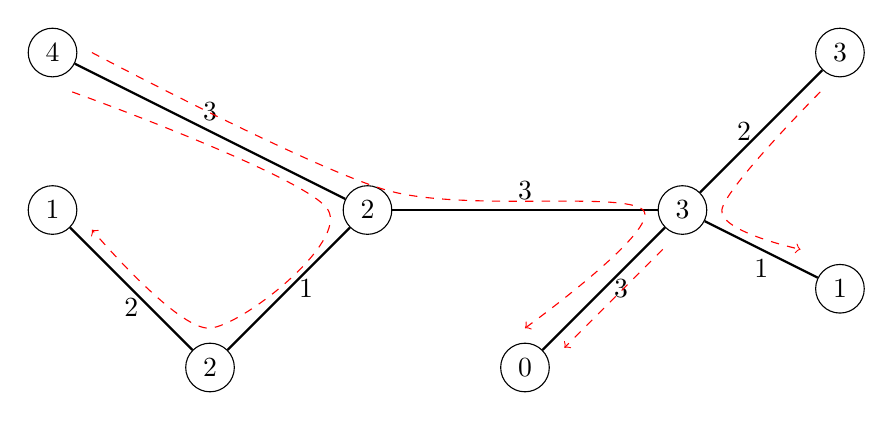
\begin{tikzpicture}
    \def \Nodes {
      1/0/4/4,
      2/4/2/2,
      3/2/0/2,
      4/0/2/1,
      5/8/2/3,
      6/10/4/3,
      7/10/1/1,
      8/6/0/0}
    \def \Edges {
      1/2/3/above,
      2/3/1/right,
      3/4/2/below,
      2/5/3/above,
      5/6/2/left,
      5/7/1/below,
      5/8/3/right}

    \foreach \id / \x / \y / \w in \Nodes {
      \node[draw,circle] (\id) at (\x, \y) {$\w$};
    }
    \foreach \x / \y / \w / \labelpos in \Edges {
      \path[draw,-,thick] (\x) -- (\y) node[midway,\labelpos] {$\w$};
    }

    \draw [red,->,dashed] plot [smooth] coordinates {(0.25,3.5) (3.5,2) (2,0.5) (0.5,1.75)};
    \draw [red,->,dashed] plot [smooth] coordinates {(0.5,4) (4.25,2.25) (7.5,2.0) (6,0.5)};
    \draw [red,->,dashed] plot [smooth] coordinates {(9.75,3.5) (8.5,2) (9.5,1.5)};
    \draw [red,->,dashed] plot [smooth] coordinates {(7.75,1.5) (6.5,0.25)};
  \end{tikzpicture}
\end{figure}

\subsection{輸入格式}

\begin{format}
\f{
$n$ $k$
$w_1$ $w_2$ $\cdots$ $w_n$
$u_1$ $v_1$ $d_1$
$u_2$ $v_2$ $d_2$
$\vdots$
$u_{n-1}$ $v_{n-1}$ $d_{n-1}$
}
\end{format}

\begin{itemize}
\tightlist
\item
  \begin{math}n\end{math} 代表自行車租借站數量
\item
  \begin{math}w_i\end{math} 代表第 \begin{math}i\end{math}
  租借站的自行車數量
\item
  第 \begin{math}i\end{math} 條道路連接租借站 \begin{math}u_i\end{math}
  與 \begin{math}v_i\end{math},且距離為 \begin{math}d_i\end{math}
\end{itemize}

\subsection{輸出格式}

\begin{format}
\f{
$D$
}
\end{format}

\begin{itemize}
\tightlist
\item
  \begin{math}D\end{math} 為整數,代表最小的調度距離總和
\end{itemize}

\subsection{測資限制}

\begin{itemize}
\tightlist
\item
  \begin{math}1 \le n \le 10^5\end{math}
\item
  \begin{math}1 \le k \le 10\end{math}
\item
  \begin{math}1 \le u_i, v_i \le n\end{math},\begin{math}u_i \neq v_i\end{math}
\item
  \begin{math}1 \le d_i \le 1000\end{math}
\item
  \begin{math}\displaystyle\sum_{i=1}^n w_i = n\times k\end{math}
\item
  \begin{math}0 \leq w_i \leq n\times k\end{math}
\item
  上述變數皆為整數
\end{itemize}

\subsection{範例測試}

\begin{example}
\exmp{
8 2
4 2 2 1 3 3 0 1
1 2 3
2 3 1
3 4 2
5 6 2
6 7 3
6 8 1
2 6 3
}{%
21
}%
\exmp{
4 3
1 10 0 1
1 4 3
3 2 2
4 2 1
}{%
16
}%
\end{example}

\subsection{評分說明}

本題共有四組子任務,條件限制如下所示。
每一組可有一或多筆測試資料,該組所有測試資料皆需答對才會獲得該組分數。

\begin{longtable}[]{@{}ccl@{}}
\toprule
子任務 & 分數 & 額外輸入限制 \\
\midrule
\endhead
1 & \(10\) & \begin{math}n \le 100\end{math} \\
2 & \(11\) & 自行車數量超過 \begin{math}k\end{math}
的租借站數量恰有一個 \\
3 & \(17\) & 所有租借站位於一條直線上,如範例 2 \\
4 & \(62\) & 無額外限制 \\
\bottomrule
\end{longtable}

\section{2022 (2022)}

\subsection{問題描述}

給定兩正整數 \begin{math}n_0\end{math} 與
\begin{math}n_2\end{math},請輸出兩正整數 \begin{math}a\end{math} 與
\begin{math}b\end{math},滿足下列條件:

\begin{enumerate}
\def\labelenumi{\arabic{enumi}.}
\tightlist
\item
  \begin{math}a\end{math} 與 \begin{math}b\end{math} 的十進位表示皆恰由
  \begin{math}n_0\end{math} 個 \begin{math}0\end{math} 與
  \begin{math}n_2\end{math} 個 \begin{math}2\end{math} 組成,其中
  \begin{math}0\end{math} 可以放在最高位(即允許 leading zeros)。
\item
  \begin{math}a\end{math} 與 \begin{math}b\end{math} 皆為
  \begin{math}22\end{math} 的倍數。
\item
  \begin{math}a\end{math}
  為符合上述條件的正整數中「第二大」的,\begin{math}b\end{math}
  為符合上述條件的正整數中「第二小」的;若符合上述條件的正整數不到
  \begin{math}2\end{math} 個,則直接輸出 \begin{math}-1\end{math}。
\end{enumerate}

舉例來說,若
\begin{math}n_0 = 1\end{math},\begin{math}n_2 = 2\end{math},則可能的
\begin{math}22\end{math} 的倍數有 \begin{math}220\end{math} 以及
\begin{math}022\end{math},第二大的為
\begin{math}022\end{math},第二小的為
\begin{math}220\end{math},故輸出為 \begin{math}022\end{math} 與
\begin{math}220\end{math}。 若
\begin{math}n_0 = 2\end{math},\begin{math}n_2 = 1\end{math},則沒有任何可能的
\begin{math}22\end{math} 的倍數,故輸出為 \begin{math}-1\end{math}。

注意,一個非負整數 \begin{math}n\end{math} 為 \begin{math}22\end{math}
的倍數,若且唯若 \begin{math}n\end{math} 同時為 \begin{math}2\end{math}
與 \begin{math}11\end{math} 的倍數,而 \begin{math}11\end{math}
的倍數判別法為「奇位數的和 \begin{math}-\end{math} 偶位數的和」也是
\begin{math}11\end{math} 的倍數。

\subsection{輸入格式}

\begin{format}
\f{
$n_0$ $n_2$
}
\end{format}

\begin{itemize}
\tightlist
\item
  \begin{math}n_0\end{math} 與 \begin{math}n_2\end{math} 分別代表
  \begin{math}0\end{math} 與 \begin{math}2\end{math} 的位數
\end{itemize}

\subsection{輸出格式}

如果有兩個以上的解,請輸出

\begin{format}
\f{
$a$
$b$
}
\end{format}

其中 \begin{math}a\end{math} 與 \begin{math}b\end{math} 皆為
\begin{math}n_0+n_2\end{math} 位數;否則請輸出

\begin{format}
\f{
$-1$
}
\end{format}

\subsection{測資限制}

\begin{itemize}
\tightlist
\item
  \begin{math}1 \le n_0 \le 10^5\end{math}
\item
  \begin{math}1 \le n_2 \le 10^5\end{math}
\item
  輸入的數皆為整數
\end{itemize}

\subsection{範例測試}

\begin{example}
\exmp{
1 2
}{%
022
220
}%
\exmp{
2 1
}{%
-1
}%
\end{example}

\subsection{評分說明}

本題共有五組子任務,條件限制如下所示。
每一組可有一或多筆測試資料,該組所有測試資料皆需答對才會獲得該組分數。

\begin{longtable}[]{@{}ccl@{}}
\toprule
子任務 & 分數 & 額外輸入限制 \\
\midrule
\endhead
1 & \(8\) & \begin{math}n_0\le10\end{math} 且
\begin{math}n_2\le10\end{math} \\
2 & \(7\) & \begin{math}n_0\le30\end{math} 且
\begin{math}n_2\le30\end{math} \\
3 & \(17\) & \begin{math}n_0\le300\end{math} 且
\begin{math}n_2\le300\end{math} \\
4 & \(24\) & \begin{math}n_2\end{math} 為偶數 \\
5 & \(44\) & 無額外限制 \\
\bottomrule
\end{longtable}

\section{間諜 (spy)}

\subsection{問題描述}

身為間諜的羅伊德這次的任務是要來探查以棋盤狀城鎮規劃聞名的 TOI 王國,
王國內一共有 \begin{math}nm\end{math} 個城鎮,
很有特色地,這些城鎮恰好排成 \begin{math}n\end{math} 列
\begin{math}m\end{math} 行的棋盤狀。 在這裡我們用
\begin{math}(x, y)\end{math} 來表示第 \begin{math}x\end{math} 列第
\begin{math}y\end{math}
行城鎮的座標(\begin{math}1 \le x \le n, 1 \le y \le m\end{math})。

為了能有效率地探查整個王國,羅伊德會選擇其中一個城鎮作為起點,
並希望不重複地拜訪所有其它城鎮再回到原起點城鎮。
擁有偵查黑科技的他可以在一單位的時間從一個城鎮移動到王國內的任意其它城鎮,
並且可以在很短的時間內探查完所在城鎮的情報,
因此除了移動時間外,其他動作的耗時都可以視為 \begin{math}0\end{math}
忽略不計。

但不幸的是 TOI 王國早已知道預謀並已在各城鎮裝設監視器,
當他們在某個城鎮發現間諜的蹤跡後,
將會把全國的警力集中,並在羅伊德抵達下一個城鎮前(下一個單位的時間)將所有警力分配至\textbf{所有與上個城鎮同行、同列或者同對角線}的城鎮加強巡邏。
(註:我們說 \begin{math}(x_1, y_1), (x_2, y_2)\end{math}
在同一對角線,若且惟若 \begin{math}|x_1 - x_2| = |y_1 - y_2|\end{math})
為了避免被王國的警衛抓到,
羅伊德想在避開增強警力城鎮的前提下找出一條路線拜訪所有城鎮並回到原起點,請問該怎麼做呢?

\subsection{輸入格式}

\begin{format}
\f{
$n$ $m$
}
\end{format}

\begin{itemize}
\tightlist
\item
  \begin{math}n\end{math} 代表王國城鎮列數,\begin{math}m\end{math}
  代表行數
\end{itemize}

\subsection{輸出格式}

若存在可以避開巡邏,中途不重複拜訪任一城鎮並回到原點的路徑,請輸出任意一條這樣的路徑。
一條符合要求的路徑應依照下列格式輸出依序經過的城鎮編號:

\begin{format}
\f{
$x_1$ $y_1$
$x_2$ $y_2$
$\vdots$
$x_{nm}$ $y_{nm}$
$x_1$ $y_1$
}
\end{format}

\begin{itemize}
\tightlist
\item
  第 \begin{math}i\end{math} 個訪問的城鎮座標為
  \begin{math}(x_i, y_i)\end{math},其中\begin{math}x_i, y_i\end{math}
  都是整數
\item
  若有以下任意一個條件不符,將會得到 Wrong Answer

  \begin{itemize}
  \tightlist
  \item
    前 \begin{math}nm\end{math} 個座標有重複或不存在的座標
  \item
    \begin{math}(x_i, y_i)\end{math} 與
    \begin{math}(x_{i+1}, y_{i+1})\end{math},或者
    \begin{math}(x_{nm}, y_{nm})\end{math} 與
    \begin{math}(x_1, y_1)\end{math} 位於同一行、列或對角線上
  \end{itemize}
\item
  行尾空白、換行位置並不影響答案正確性,但請勿輸出多餘的資訊
\end{itemize}

若不存在符合要求的路徑,請輸出:

\begin{format}
\f{
-1
}
\end{format}

\subsection{測資限制}

\begin{itemize}
\tightlist
\item
  \begin{math}2 \le n, m \le 1000\end{math}
\item
  \begin{math}4 \le nm \le 2000\end{math}
\item
  上述變數皆為整數
\end{itemize}

\subsection{範例測試}

\begin{example}
\exmp{
3 3
}{%
-1
}%
\exmp{
4 3
}{%
4 2
2 1
3 3
1 2
3 1
4 3
2 2
4 1
1 3
3 2
1 1
2 3
4 2
}%
\end{example}

\subsection{評分說明}

本題共有四組子任務,條件限制如下所示。
每一組可有一或多筆測試資料,該組所有測試資料皆需答對才會獲得該組分數。

\begin{longtable}[]{@{}ccl@{}}
\toprule
子任務 & 分數 & 額外輸入限制 \\
\midrule
\endhead
1 & \(7\) & \begin{math}nm \le 16\end{math} \\
2 & \(35\) & \begin{math}n = 2\end{math} 或
\begin{math}m = 2\end{math} \\
3 & \(47\) & \begin{math}n \ge 12\end{math} 且
\begin{math}m \ge 12\end{math} \\
4 & \(11\) & 無額外限制 \\
\bottomrule
\end{longtable}
